\begin{frame}
\frametitle{I do not believe in neutrinos}
\begin{columns}
\column{0.35\textwidth}
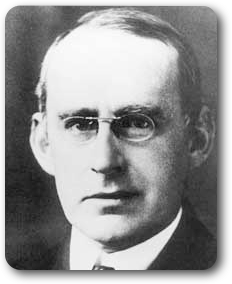
\includegraphics[scale=0.3]{img/eddington.png}
 
 \column{0.6\textwidth}
%\begin{block}{}
Sir Arthur Eddington: ``Just now nuclear physicists are writing a great deal about hypothetical particles called neutrinos supposed to account for certain peculiar facts observed in $\beta$-ray disintegration. We can perhaps best describe the neutrinos as little bits of spin-energy that have got detached. I am not much impressed by the neutrino theory. \alert{In an ordinary way I might say that I do not believe in neutrinos}... But I have to reflect that a physicist may be an artist, and you never know where you are with artists. My old-fashioned kind of disbelief in neutrinos is scarcely enough. \alert{Dare I say that experimental physicists will not have sufficient ingenuity to make neutrinos?"}

%\end{block}
\end{columns}
\end{frame}

\begin{frame}
\frametitle{The discovery of neutrinos}

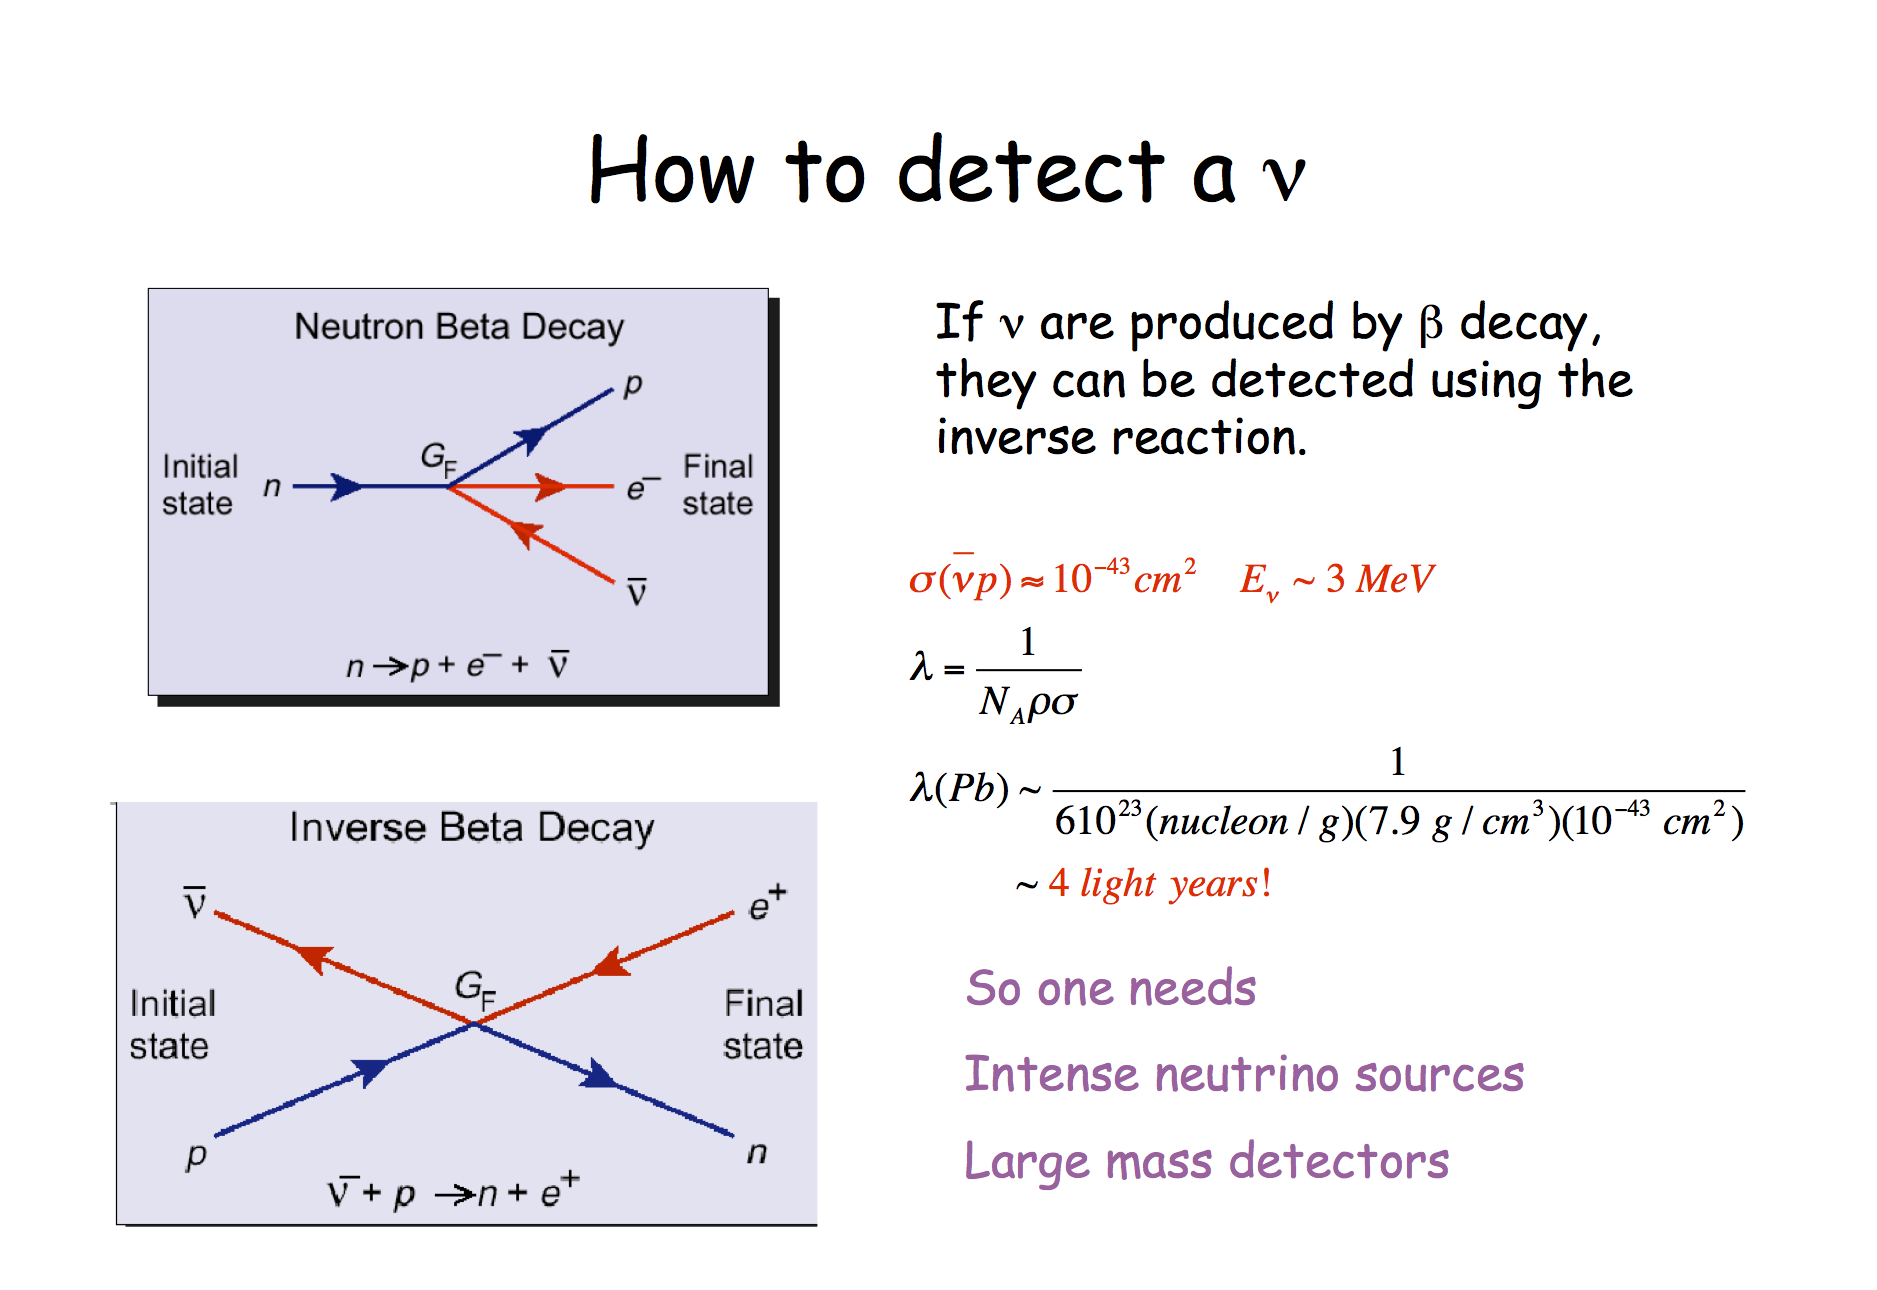
\includegraphics[scale=0.3]{img/DetectNeutrinos.png}

\end{frame}

\begin{frame}

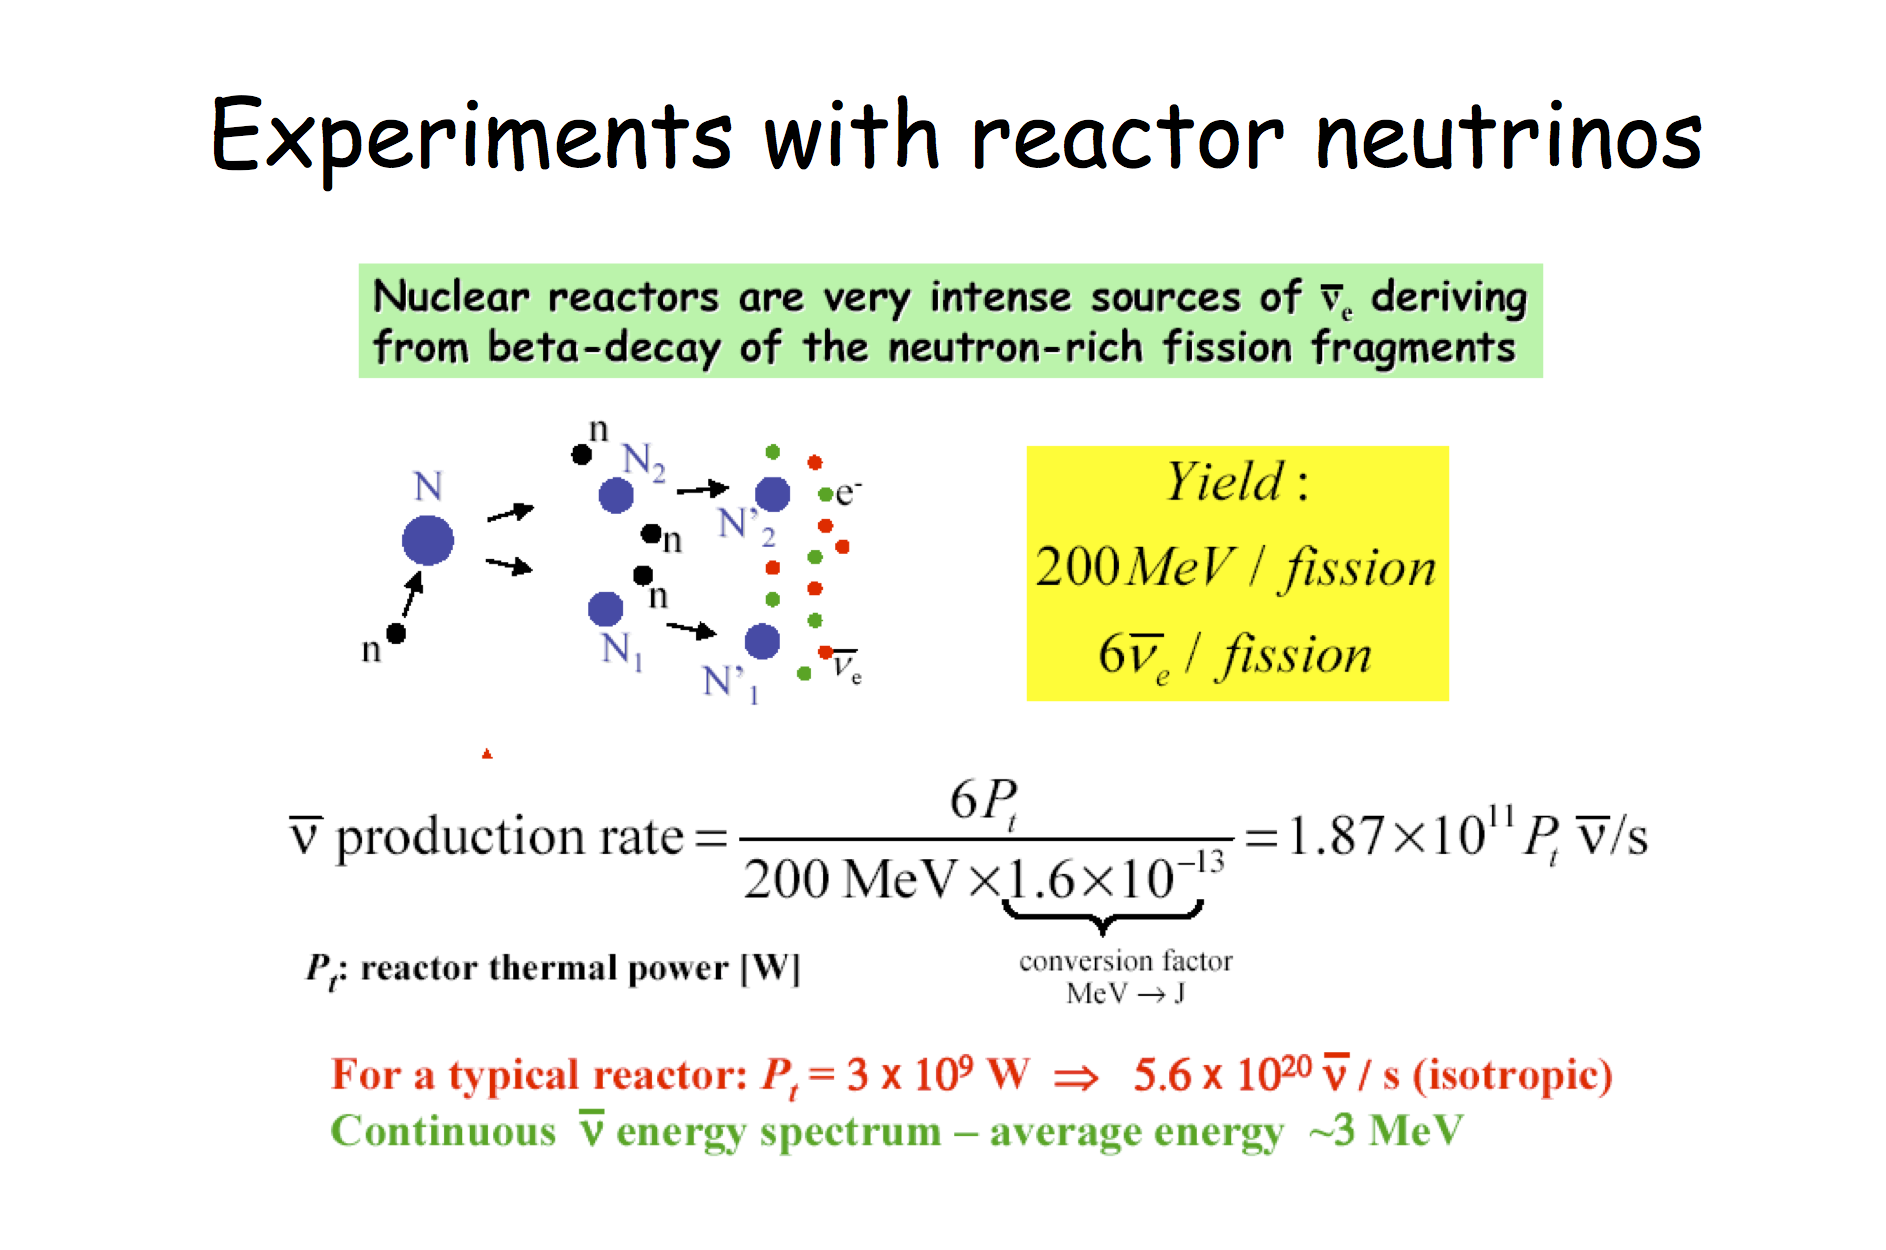
\includegraphics[scale=0.35]{img/ReactorNeutrinos.png}

\end{frame}

\begin{frame}
\frametitle{Reines, Cowen and delayed neutrons}
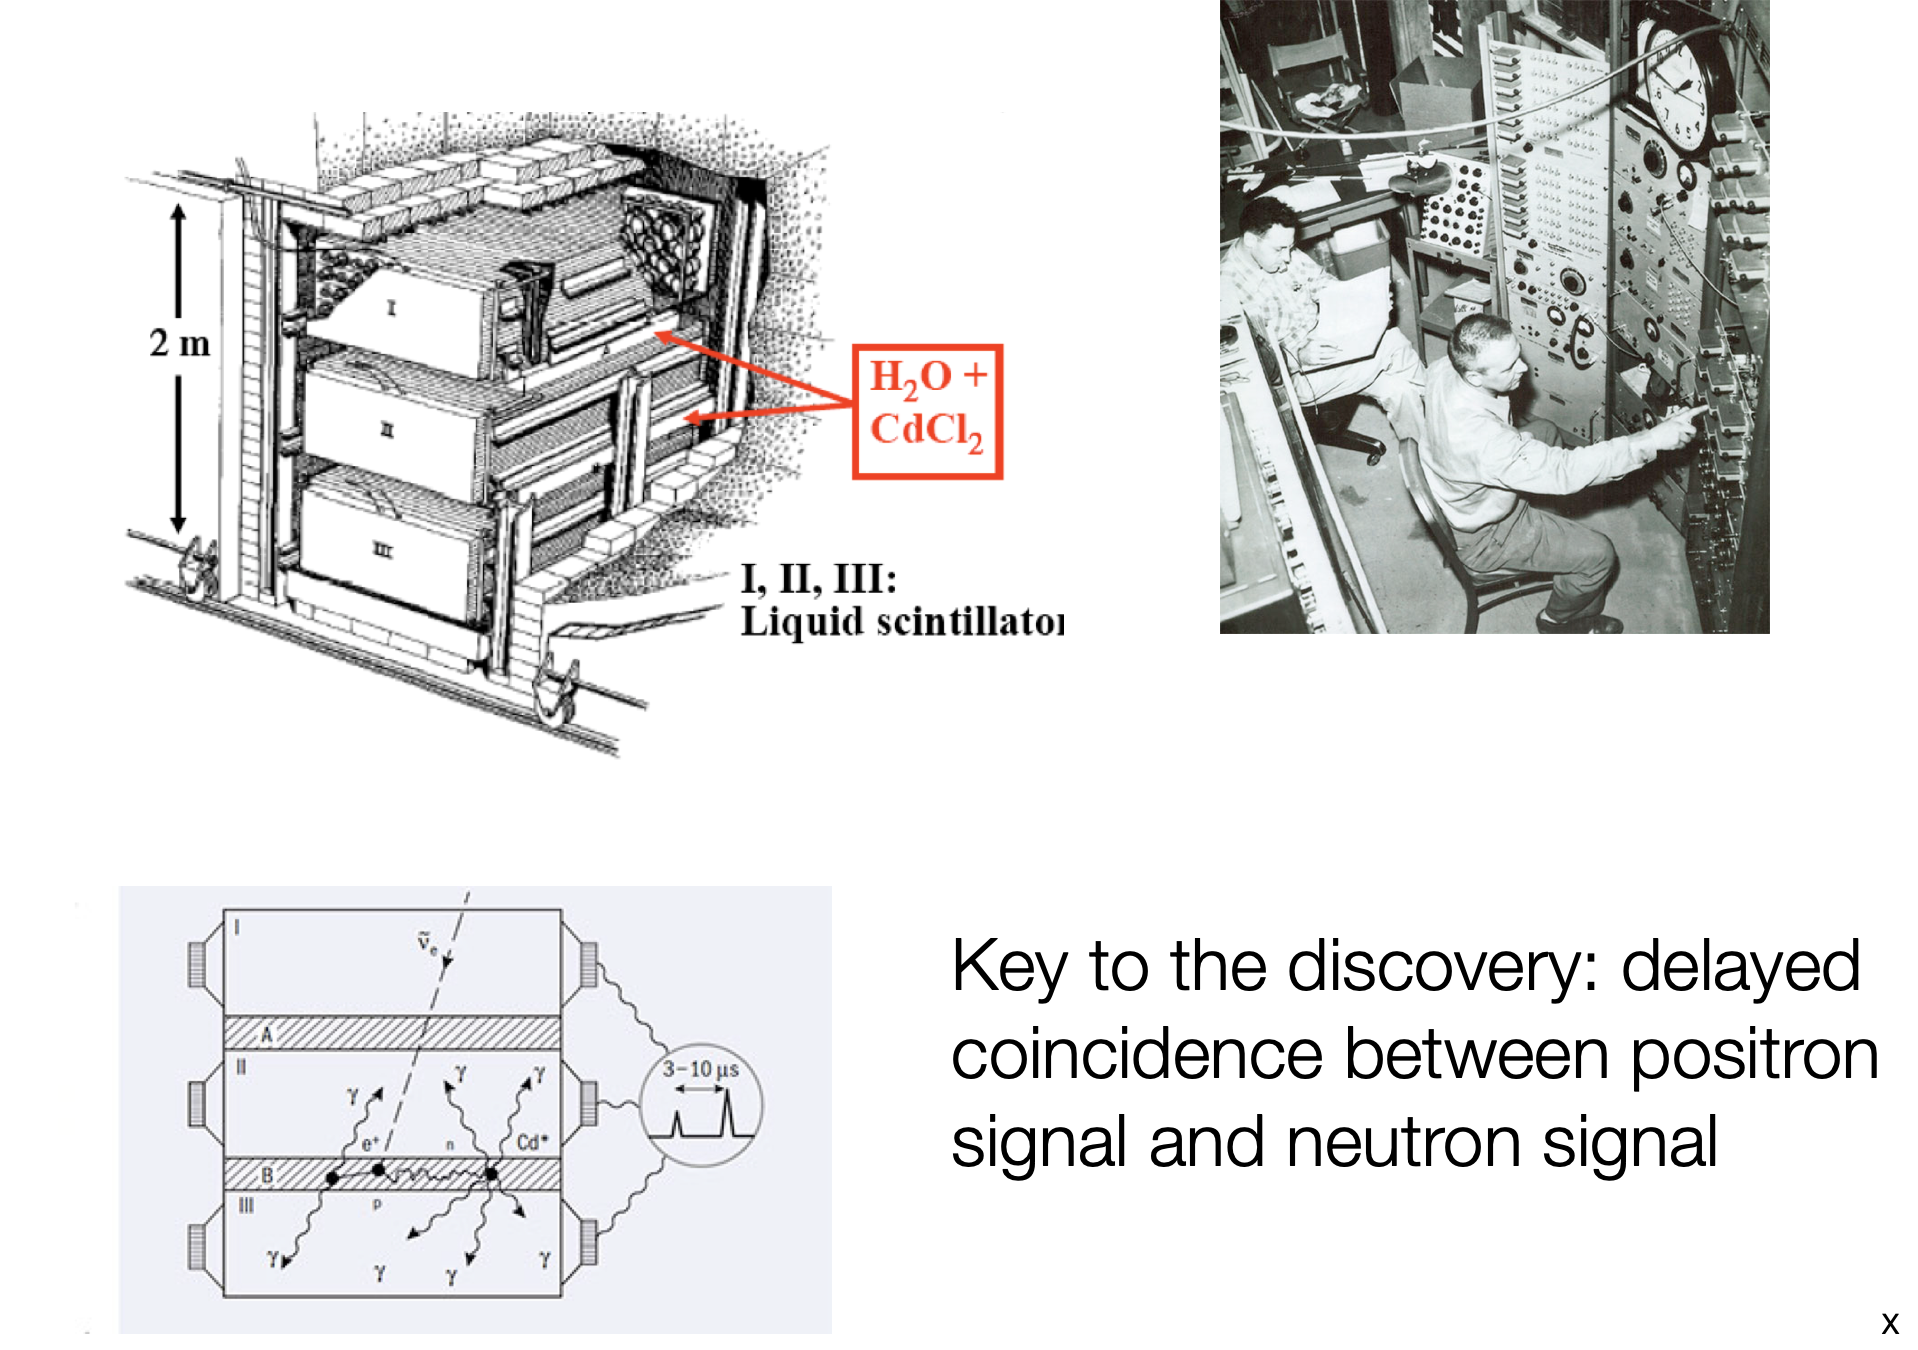
\includegraphics[scale=0.35]{img/ReinesCowen.png}

\end{frame}

%\begin{frame}
%
%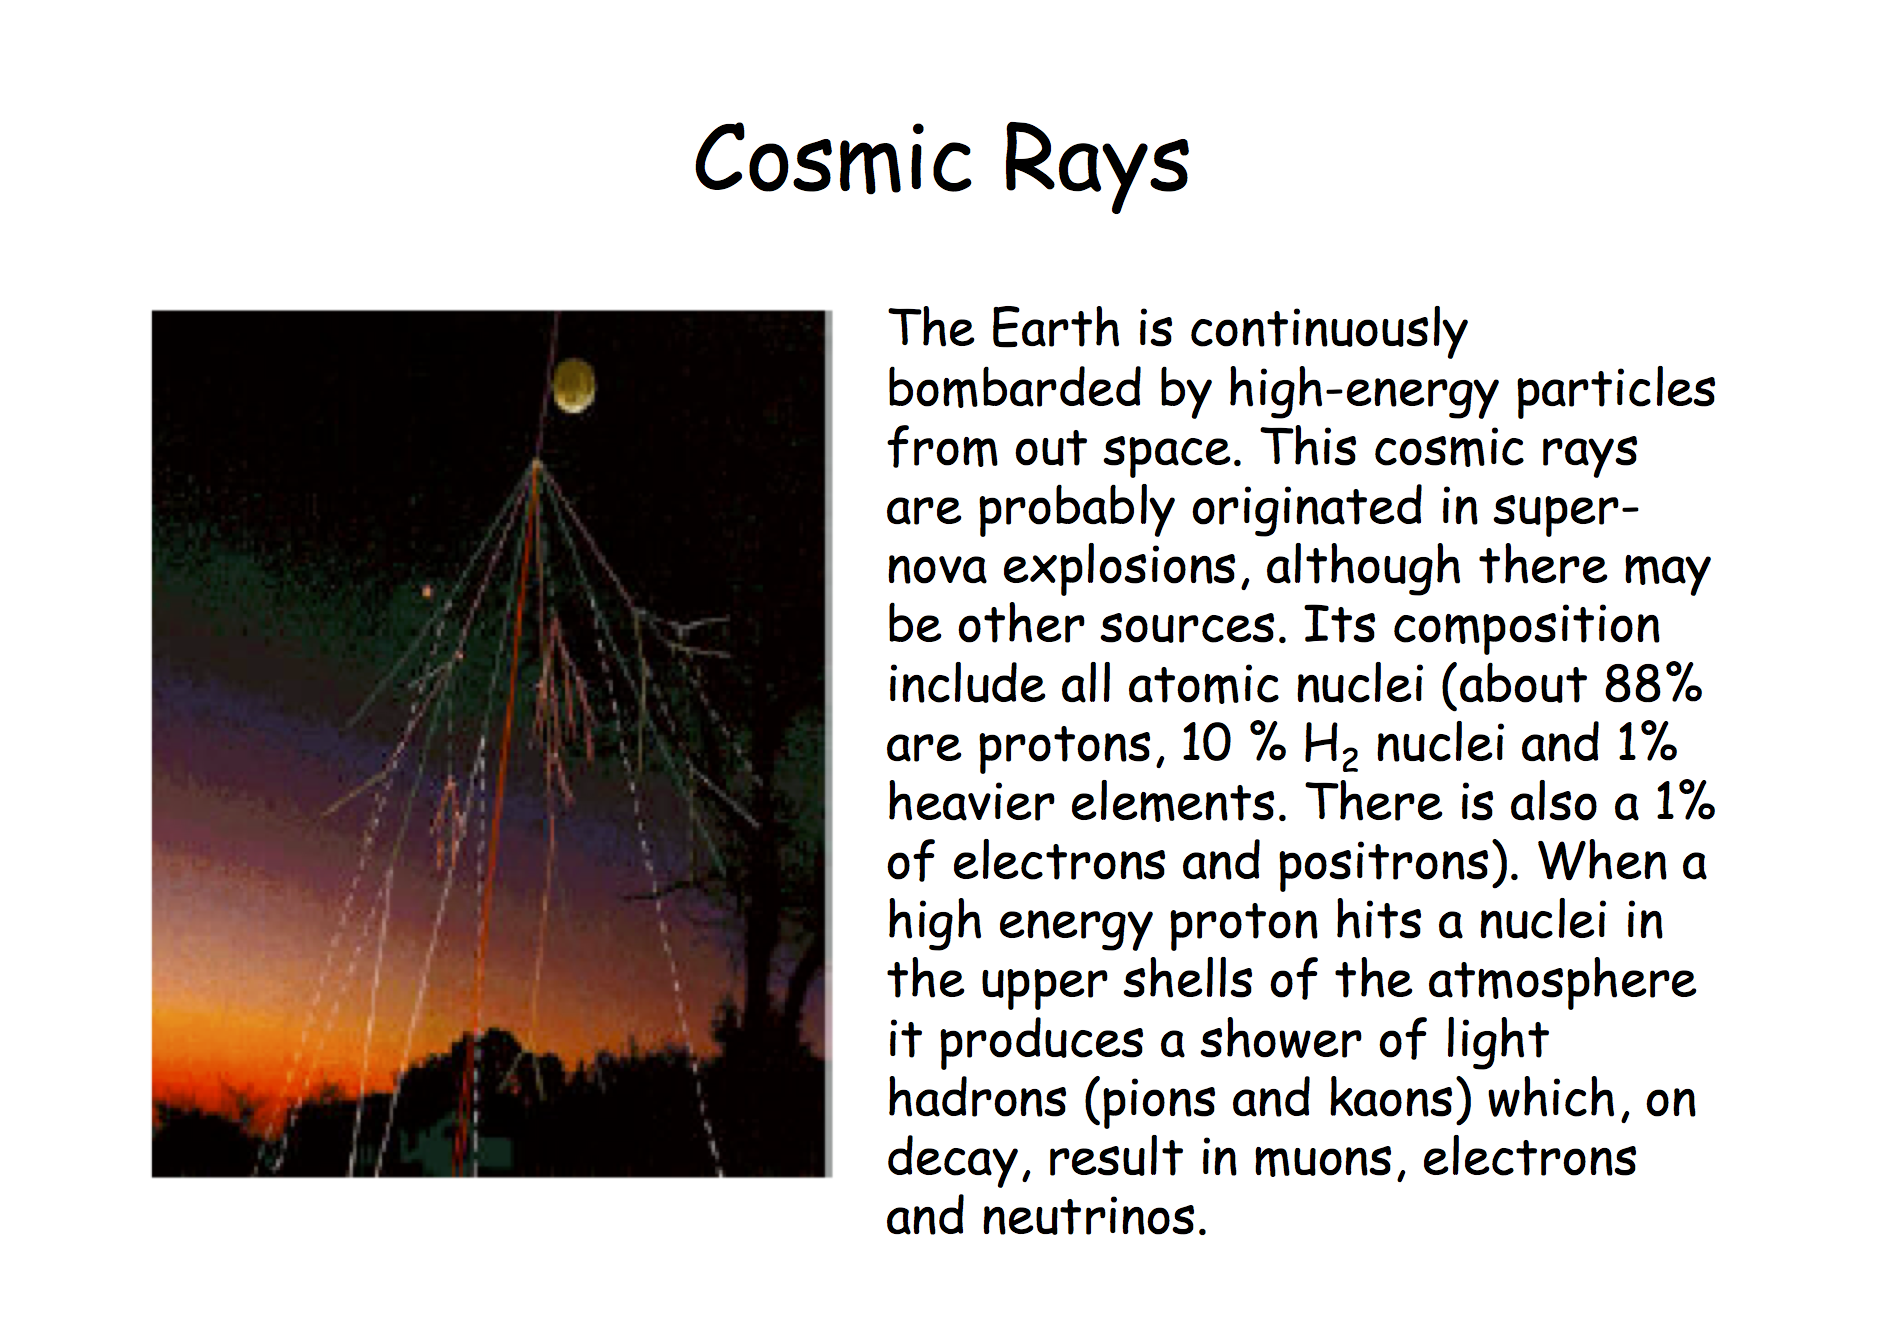
\includegraphics[scale=0.35]{CosmicRays.png}
%
%\end{frame}
%\begin{frame}
%
%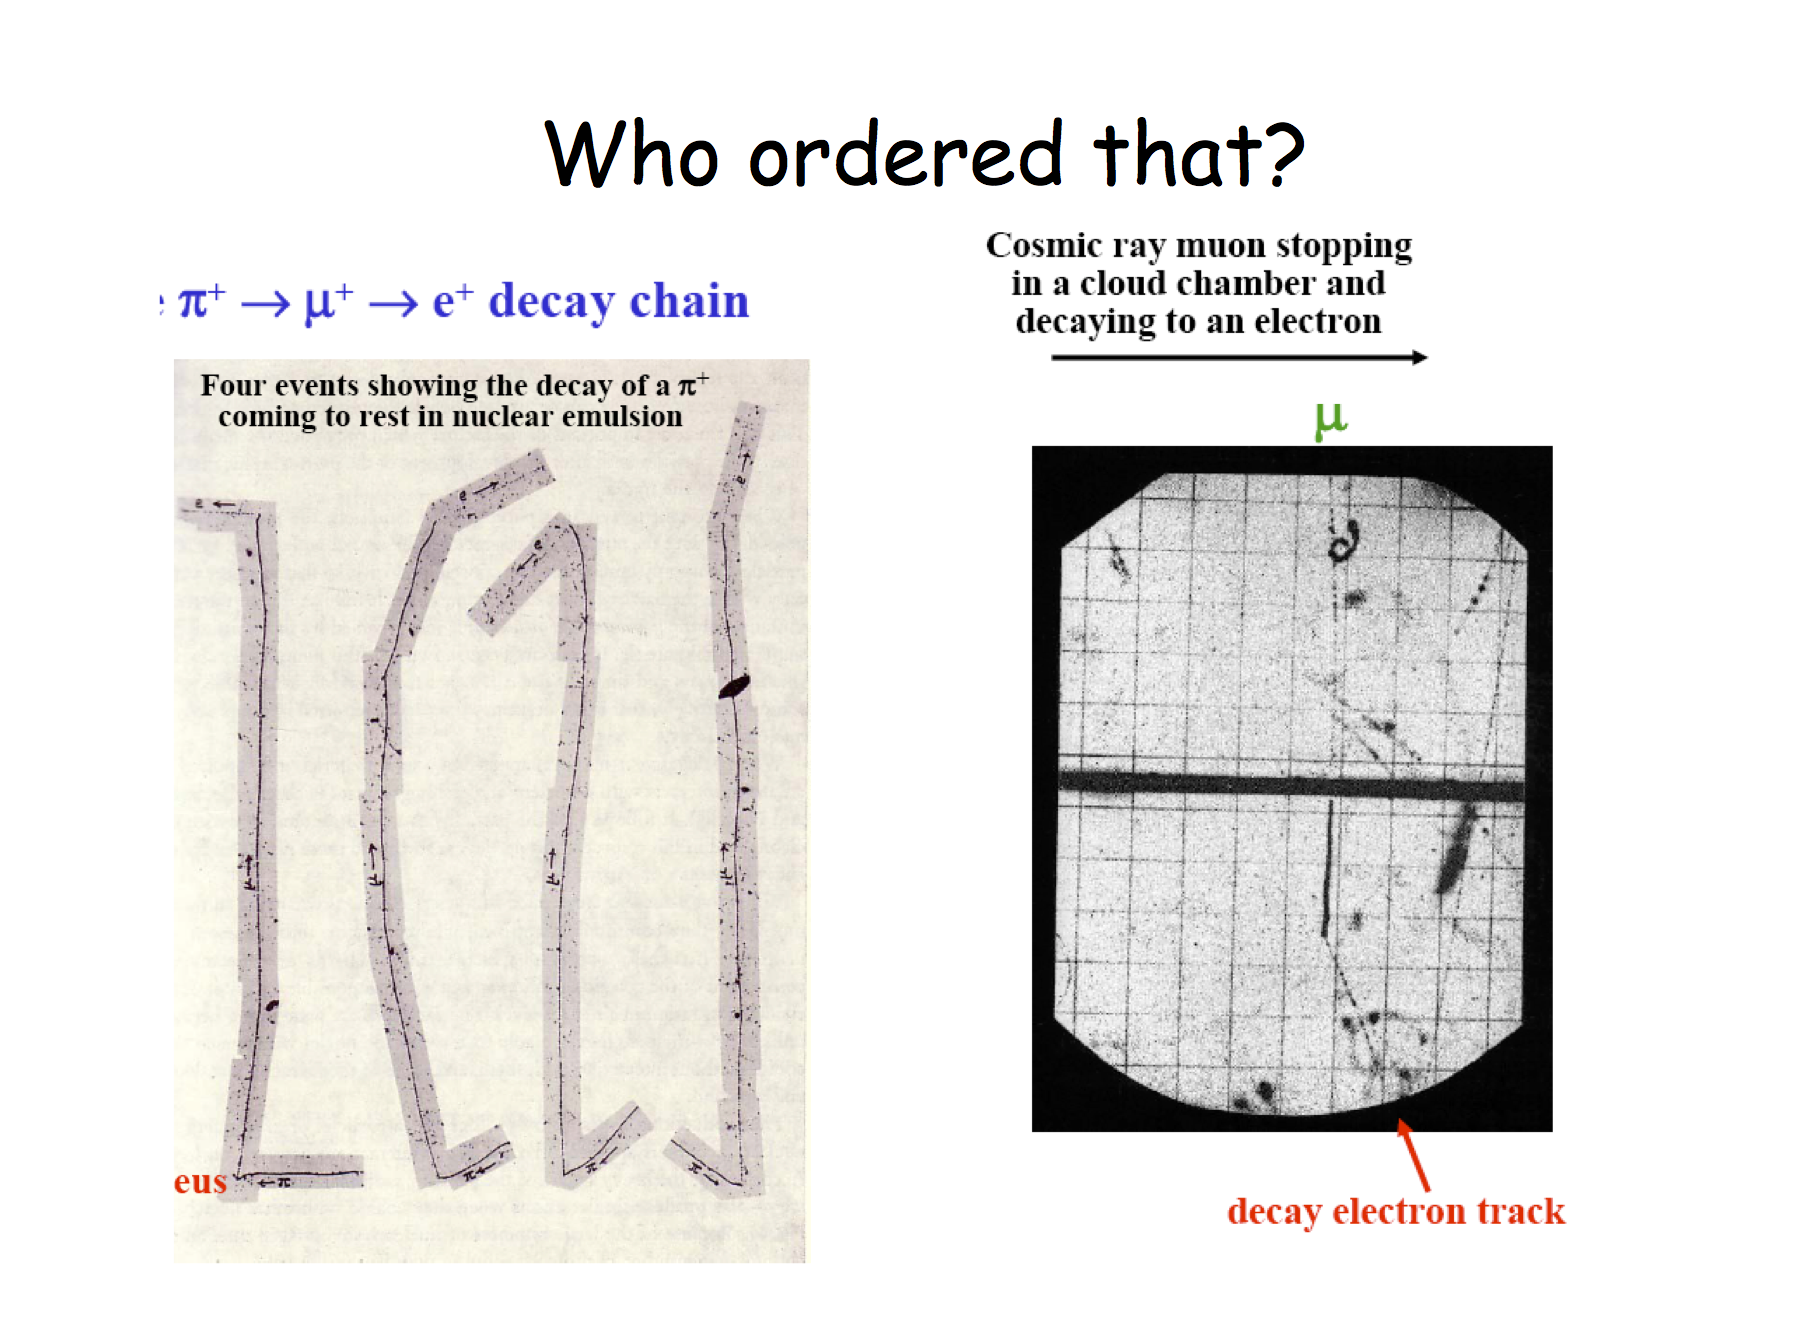
\includegraphics[scale=0.35]{WhoOrderedThat.png}
%
%\end{frame}
%\begin{frame}
%
%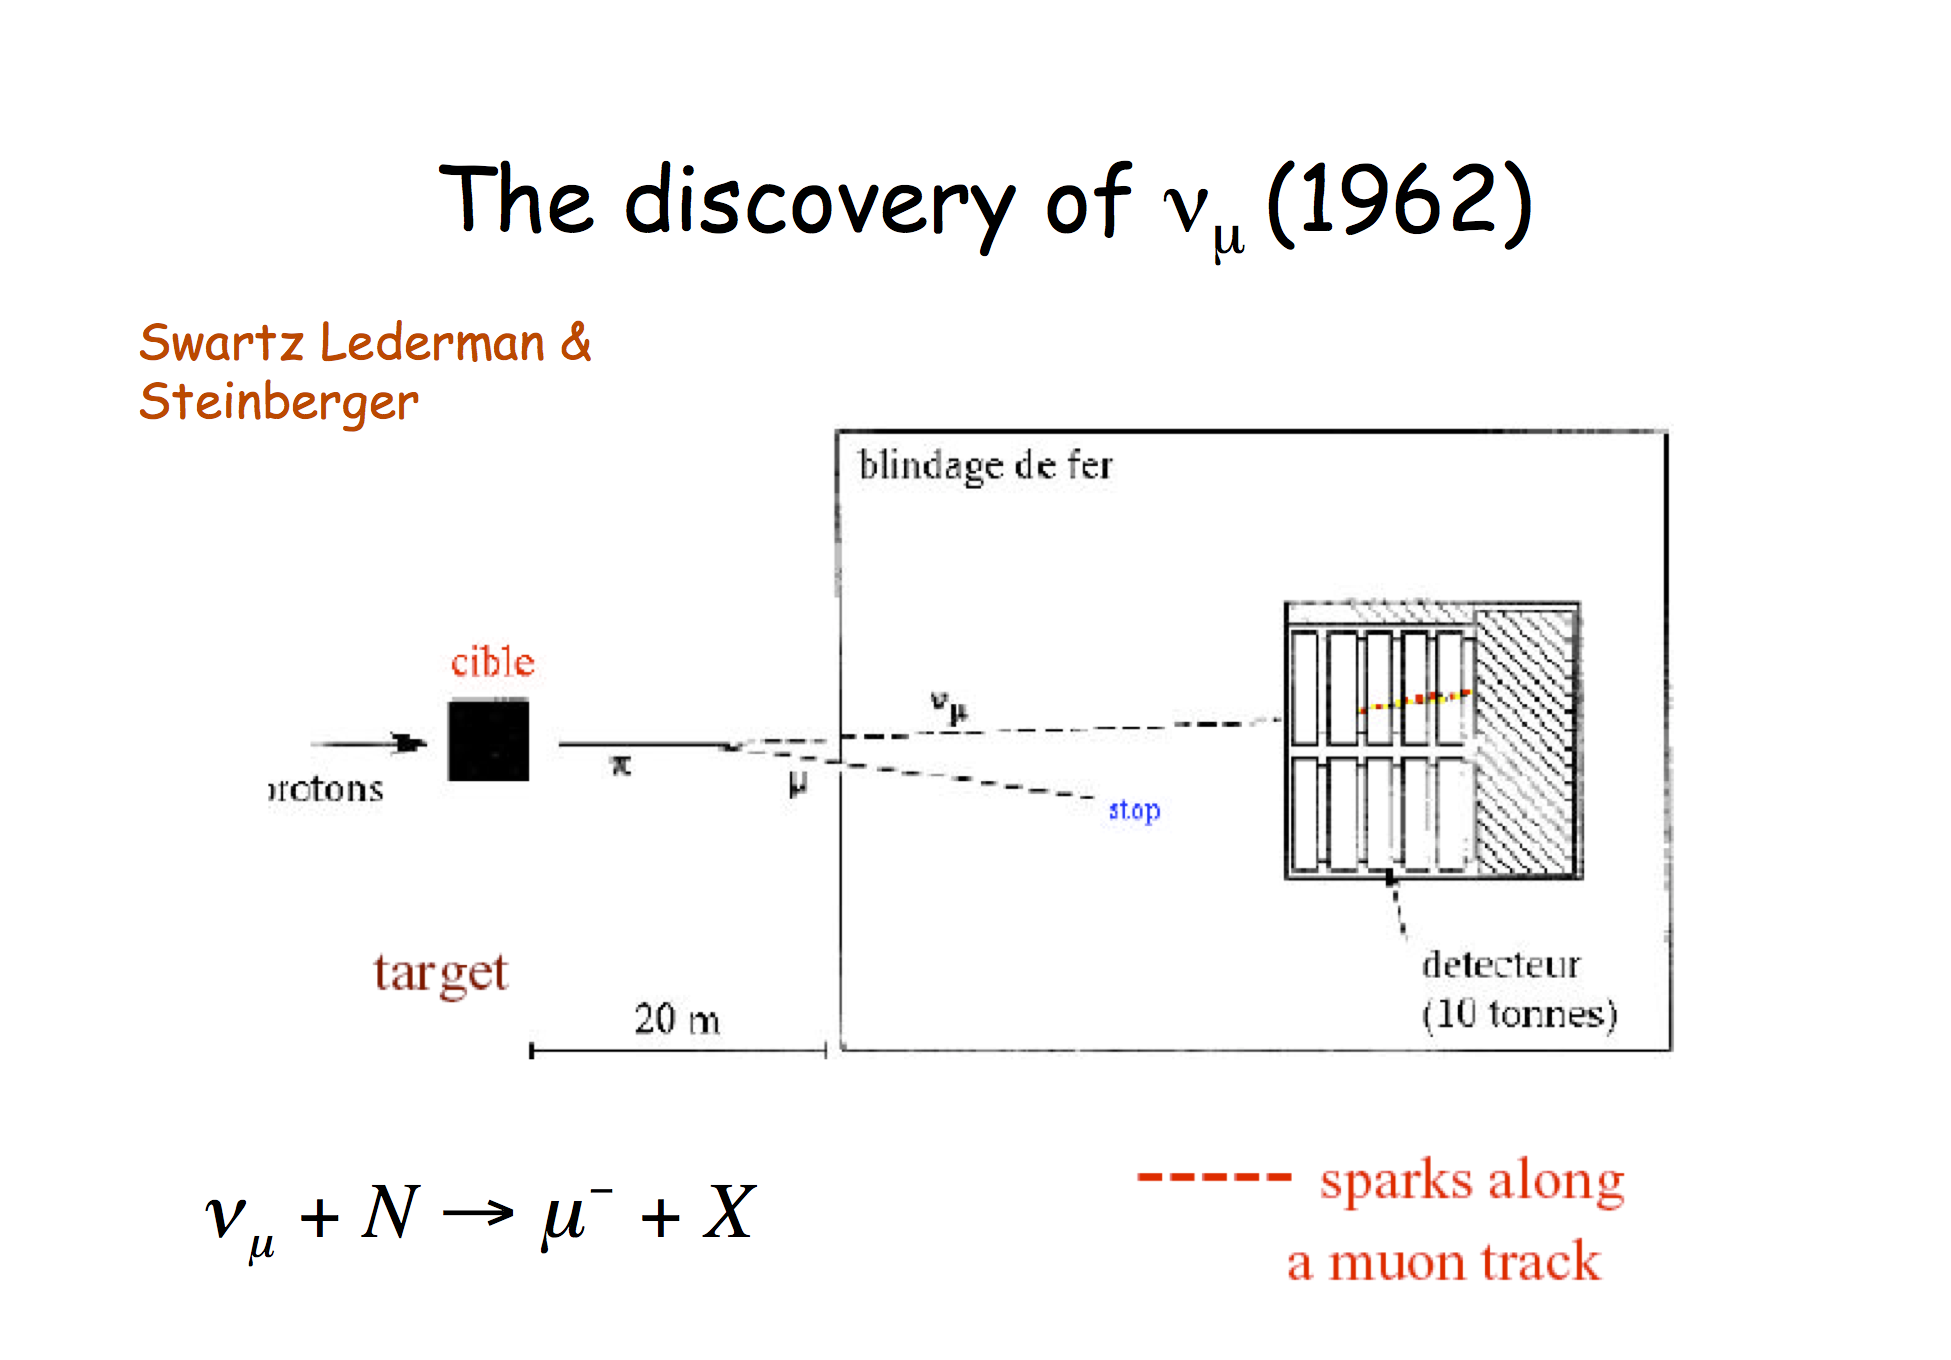
\includegraphics[scale=0.35]{DiscoveryNumu.png}
%
%\end{frame}
%\begin{frame}
%
%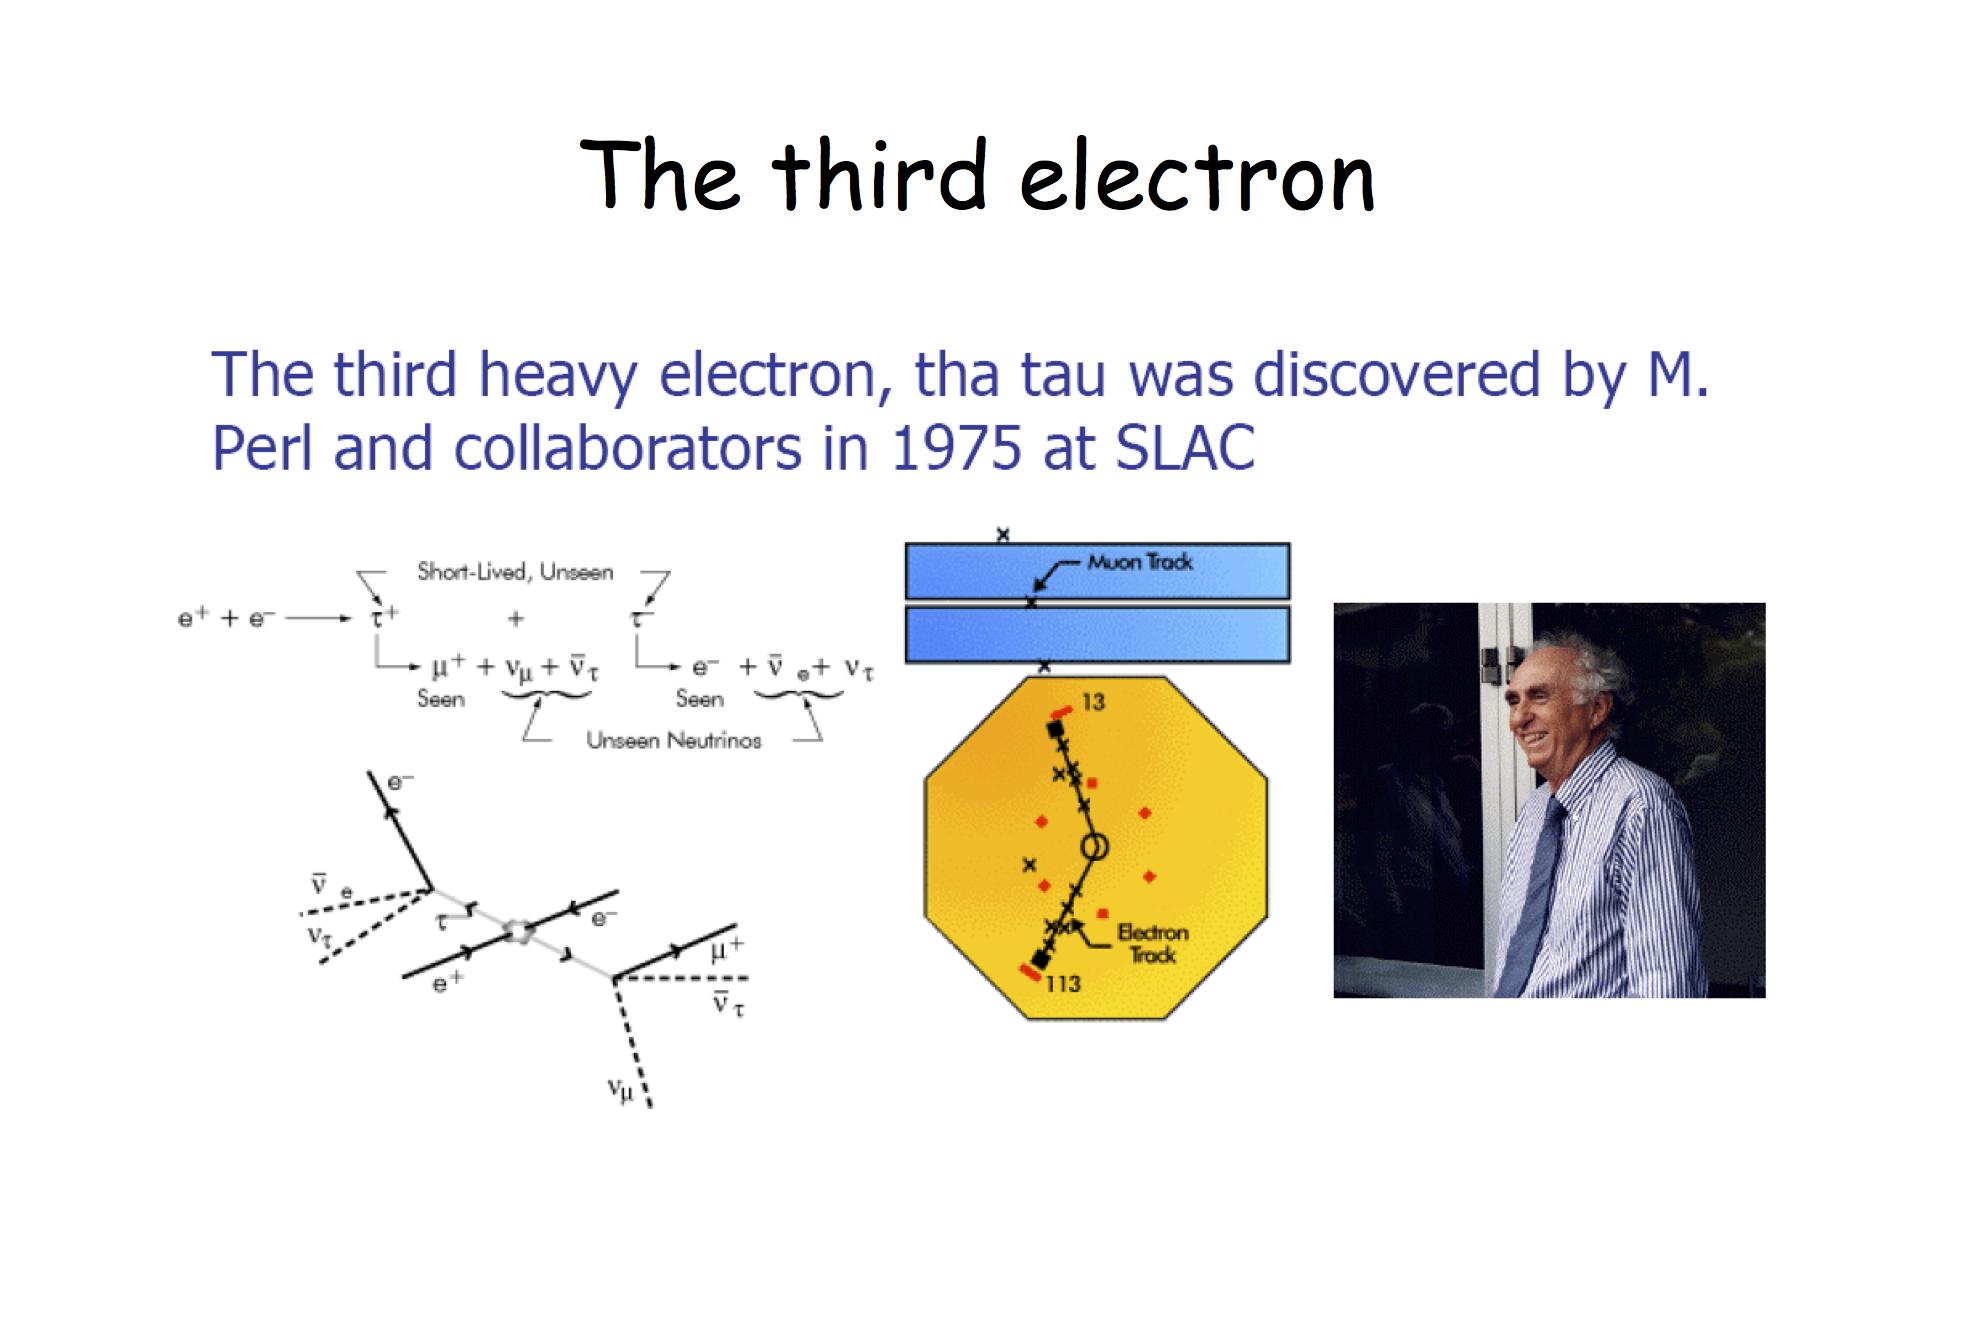
\includegraphics[scale=0.35]{tau.png}
%
%\end{frame}
%\begin{frame}
%
%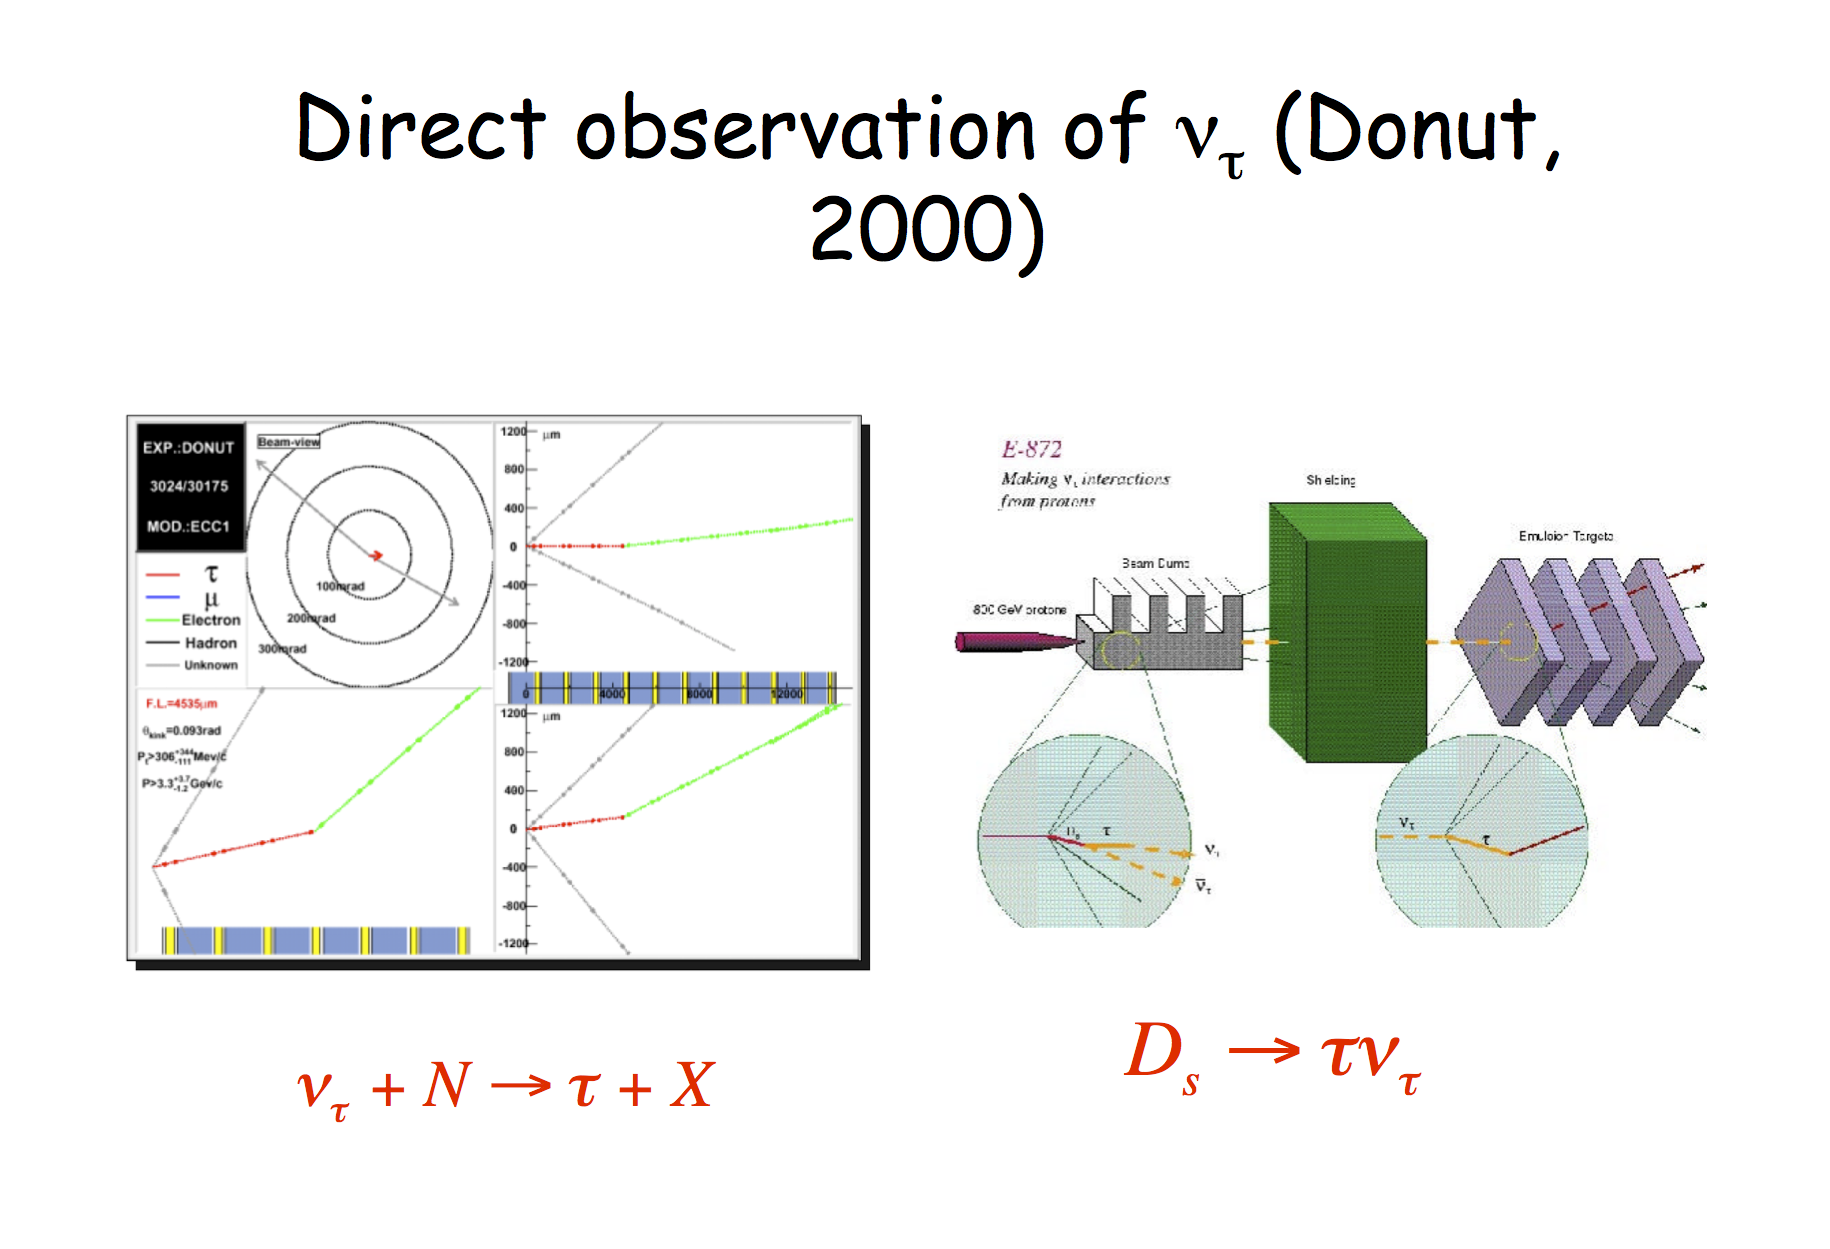
\includegraphics[scale=0.35]{DirectNuTau.png}
%
%\end{frame}
\begin{frame}
\frametitle{Neutrinos everywhere}
\begin{columns}
\column{0.35\textwidth}
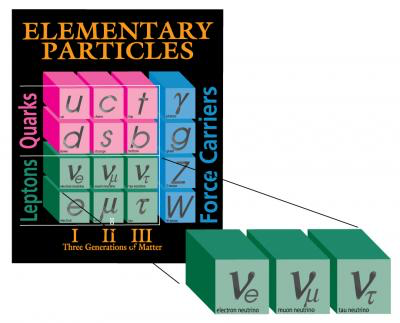
\includegraphics[scale=0.25]{img/Generations2.png}

Two heavy electrons (the $\mu$~and the $\tau$) have been discovered, each one accompanied with its own neutrino. For reasons yet unknown to us, Nature has chosen to produce three copies of the elementary fermions, identical except for their mass. 
 
 \column{0.6\textwidth}
%\begin{block}{}
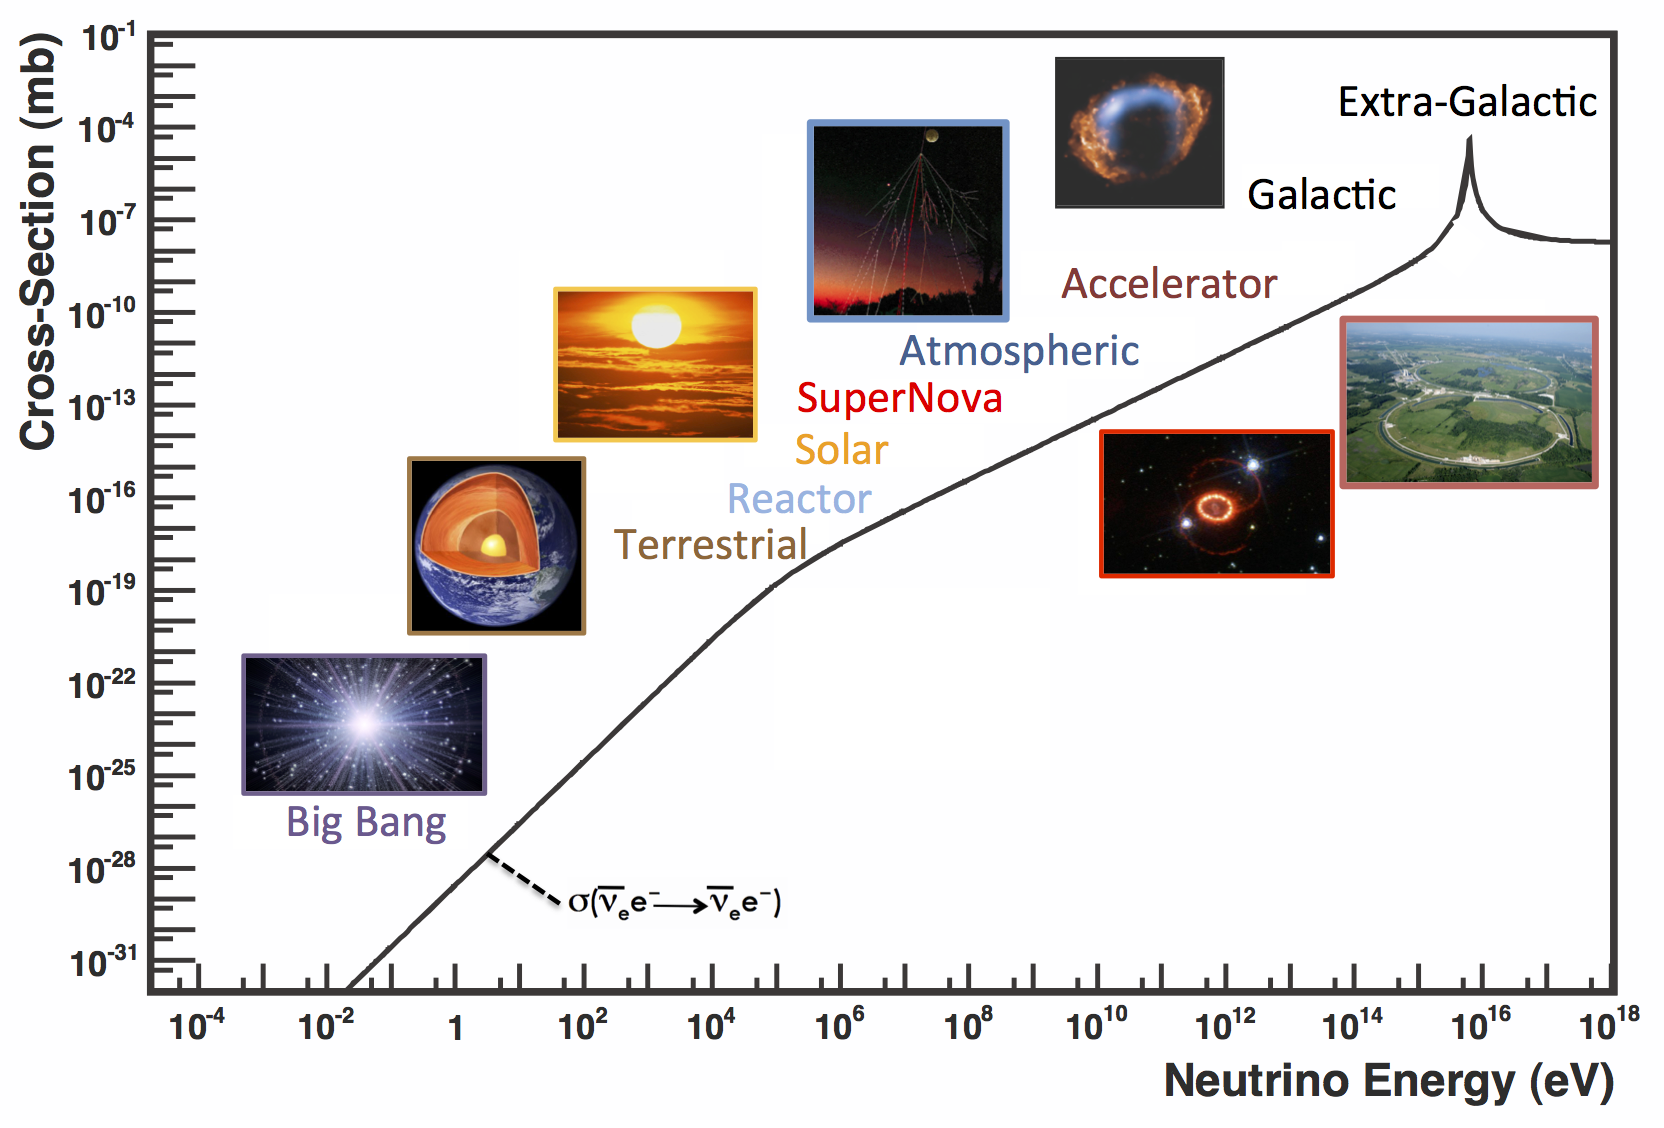
\includegraphics[scale=0.25]{img/NeutrinoSources.png}

Neutrinos are everywhere and we have produced and detected them by the millions. Eddington would not have made a living as a prophet (who does?)


%\end{block}
\end{columns}




\end{frame}

